% Section content template for individual Educative lessons
% This file contains the actual content for a specific section
% Generated from Educative API section content

% Section: Getting Ready: The Amazon Online Shopping System
% Section ID: 6076512478691328
% Section Slug: getting-ready-the-amazon-online-shopping-system
% Generated: 2025-12-12T22:44:29.274767

\subsection{Problem definition}\label{LZRzYAxZZSzGl2QhlqOXs}
\\
\textbf{Amazon} is an online retail platform that allows its users to buy from and sell products to other users. There are numerous product categories that customers can search and choose from. Products have reviews and ratings that can help customers make a buying decision. Each customer has a shopping cart where they can add products they wish to order. Once customers have added their favorite products to the cart, they can check out the cart and choose a payment method to place their orders. The customers are notified about their order and shipment statuses until the order is delivered. The system also allows users to add products they want to sell.

\begin{figure}[htbp]
 \centering
 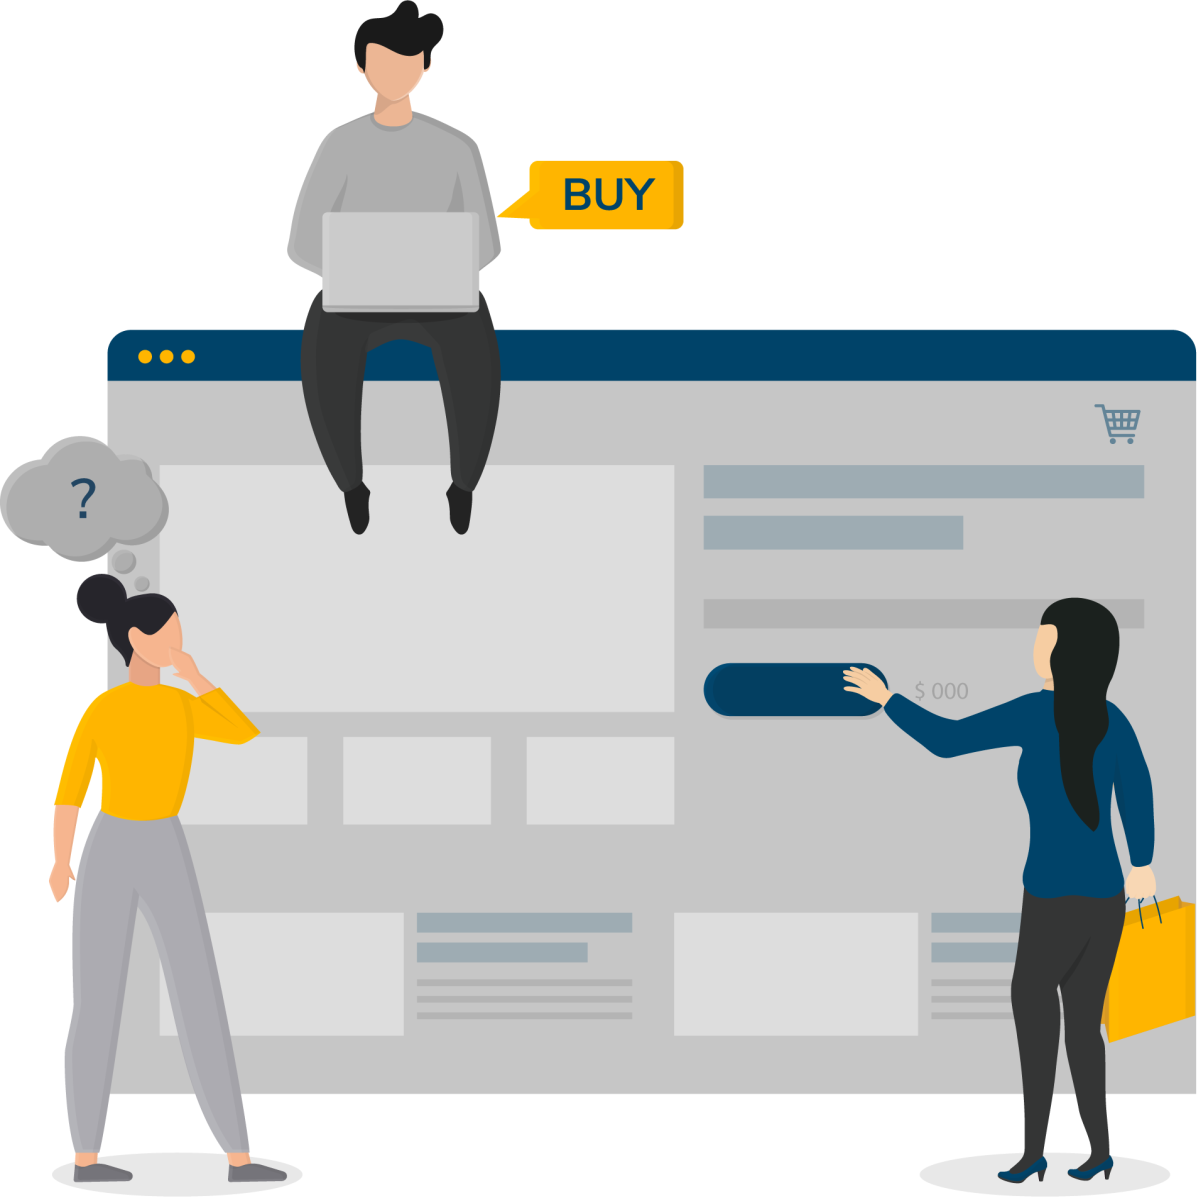
\includegraphics[width=0.15\textwidth]{Images/chapter_19/section_6076512478691328/5912623242805248.png}
 \caption{Users interacting with an online shopping system}
\end{figure}

\subsection{Expectations from the interviewee}\label{6wAj553qfBzDUjXSTZX8t}
\\
Numerous components are present in the Amazon online shopping system, each with specific constraints and requirements. The following provides an overview of some of the main things the interviewer will want to hear you discuss in more detail.

\subsubsection{Discoverability}\label{y2hvzNl33Gwxac-_LYbVK}
\\
For an online shopping system like Amazon, discoverability is one of the key features that distinguishes it from others. You can ask the following questions to know more about the system:

\begin{itemize}
\item
\protect\phantomsection\label{46HTIPR8lLlJW1bU6wwZx}
How will the buyer discover a product?
\item
\protect\phantomsection\label{0w7LQK4xRHJ7mp_JHAWpi}
How will the search surface result?
\end{itemize}

\subsubsection{Cart and checkout}\label{h7dhGrCg3emlXZdoxSxHq}
\\
One of the most significant attributes of the online shopping system is the cart and checkout functionality that it provides to its customers. The interviewer expects the cart and checkout to behave in a certain way. You may ask the interviewer:

\begin{itemize}
\item
\protect\phantomsection\label{q7KslQ3wL0UZYKsZX5XhM}
How will the design adhere to known best practices while introducing innovative checkout semantics like ``one-click purchase?''
\end{itemize}

\subsubsection{Payment methods}\label{-6IWSlTeYFphYQRYW5G1s}
\\
The interviewer expects you to ask about the payment methods to determine the necessary requirements. You may ask the following questions:

\begin{itemize}
\item
\protect\phantomsection\label{VeLJQD2phbMB1aIuQv6l3}
How will the users pay? Will they use credit cards, gift cards, and so on?
\item
\protect\phantomsection\label{MWYYabAo3FcfAavfau_UA}
How will the payment method work with the checkout process?
\end{itemize}

\subsubsection{Product reviews and ratings}\label{DZg0KiDQHri0Yq9Pl8uC-}
\\
Product reviews and ratings help customers make informed decisions regarding what to buy. Knowing how to make this feature an effective part of the system is important. You can ask the interviewer:

\begin{itemize}
\item
\protect\phantomsection\label{C43doTbiaDLxg0IhkTeAG}
When can a user post a review and a rating?
\item
\protect\phantomsection\label{1vtYO4Y7qcCGmowDxbgpK}
How are useful reviews tracked and less useful reviews deprioritized?
\end{itemize}

\subsection{Design approach}\label{sMw8unB4kHlXZCwiPVhJ1}
\\
We will design this online shopping system using the bottom-up design approach. For this purpose, we will follow the steps below:

\begin{itemize}
\item
\protect\phantomsection\label{D8wvZxSCuIon1N5vE34I-}
Identify and design the smallest components first, such as a product.
\item
\protect\phantomsection\label{yNe1qzXP8Iz7JOfH5-2QE}
Use these small components to design bigger components, like a product category that contains different products.
\item
Repeat the steps above until we design the whole system containing multiple product categories and users.
\end{itemize}

\subsection{Design pattern~}\label{gY9SBs0IidJWM770RFDjk}
\\
During an interview, it is always good practice to discuss the design patterns under which the Amazon online shopping system falls. Stating the design patterns gives the interviewer a positive impression and shows that the interviewee is well-versed in the advanced concepts of object-oriented design.
\\
Try to answer the following question. If you are not familiar with design patterns, don't worry! You can learn about them by asking, ``Define design patterns.''

\textbf{Question:}

Which design pattern(s) should be used to design an Amazon online shopping system? Please elaborate on your choice(s).

Let's explore the requirements of the online shopping system in the next lesson.

% End of section content